\documentclass[xcolor=table,aspectratio=169]{beamer} 
% to create notes:
%\documentclass[handout,notes=only]{beamer}
% to create handouts
% \documentclass[handout]{beamer}

\setcounter{errorcontextlines}{999} %for error tracking

% COLORS
  \definecolor{blue}{RGB}{0,114,178}
  \definecolor{red}{RGB}{186,12,47}
  \definecolor{yellow}{RGB}{240,228,66}
  \definecolor{green}{RGB}{0,158,115}
  \definecolor{LightSteelBlue}{rgb}{0.690,0.770,0.870}
  \definecolor{dgreen}{rgb}{0.,0.6,0.}

\mode<presentation>
{
  \usetheme{metropolis}
}

%\setbeamercolor{math text}{fg=green!50!black}
%\setbeamercolor{normal text in math text}{parent=math text}
\usepackage{amsmath,amssymb,amsfonts}
\usepackage{booktabs}
\usepackage[latin1]{inputenc}
\usepackage{colortbl}
\usepackage[english]{babel}
   \usepackage{booktabs}
    \usepackage{epstopdf}
  \usepackage{fancyref}
  \usepackage{graphicx}
%\usepackage{pstricks}
\usepackage{pifont}
  \usepackage{array}
  \usepackage{hyperref}
  \usepackage{caption}
  \usepackage{tikz}   %for nice-looking graphs
  \usepackage{pgfplots} %for nice-looking plots of data (requires tikz package)
    \pgfplotsset{compat = newest} %to use newest plot settings in pgfplot
  \usepackage{graphicx} % for inclusion of EPS graphics
  \usepackage{multicol} % Multicolumn formatting (in-line tables)
  \usepackage{multirow}
  \usepackage{rotating}  % allows for rotated tables
  \usepackage{setspace}
  \usepackage{array}     % Modifications of tabular environment
  % \usepackage{subfloat} %to put multiple floats in the same frame
  \usepackage{color}
  \usepackage{lscape}
  \usepackage[super,negative]{nth}
  \usepackage{adjustbox}
  \usepackage{collectbox}
  % \usepackage{subfig}
  \usepackage{subcaption}
  \usepackage{appendixnumberbeamer}

  %for setting font to palatino and math cmr
% \renewcommand\rmdefault{pplx}
% \renewcommand\mathfamilydefault{cmr}

%\usepackage{lmodern}
%\usepackage[T1]{fontenc}


%Bibliography options%
  \usepackage[comma]{natbib}
  \newcommand{\Cite}{\citet} % this for natbib
  \bibpunct{(}{)}{;}{a}{}{;} %set if using natbib

%\setbeamercovered{opaque}
\setbeamertemplate{navigation symbols}{} %//removes the navigation symbols
\setbeamertemplate{frametitle continuation}[from second][\insertcontinuationcountroman]  %//to eliminate Roman numerals on 'first' slide when using allowframebreaks


%
% Some useful commands
%
  \newcommand{\sw}[1]{\begin{sideways}#1\end{sideways}}
  \newcommand{\bit}{\hspace{1 em}}
  \newcommand{\rarrow}{\selectfont\ding{220}}
  \newcommand{\skiplink}{\tiny{\gray\selectfont\ding{59}}}
  \newcommand{\goback}{\Acrobatmenu{GoBack}{\gray\selectfont\ding{242}}}
  \newcommand{\x}{\selectfont\ding{52}}
  \newcommand{\verbatimsize}{\tiny}

  %for putting refs in lit review
  \newcommand{\smallref}[1]{\scriptsize {\color{gray}[#1] }\normalsize}

  %for overlays
  \newenvironment{slide}{\begin{frame}[allowframebreaks]}{\end{frame}}
  \newenvironment{refs}{\footnotesize \color{darkgray} [}
      {] \normalsize \color{black}}
  \newenvironment{stepenumerate}{\begin{enumerate}[<+->]}{\end{enumerate}}
  \newenvironment{stepitemize}{\begin{itemize}[<+->]}{\end{itemize} }
  \newenvironment{stepenumeratewithalert}{\begin{enumerate}[<+-| alert@+>]}{\end{enumerate}}
  \newenvironment{stepitemizewithalert}{\begin{itemize}[<+-| alert@+>]}{\end{itemize} }
    %% Change the bg color to adjust your transition slide background color!

	%for distinguishing sections
	\newenvironment{transitionframe}{\setbeamercolor{background canvas}{bg=LightSteelBlue}\begin{frame}}{\end{frame}}




%-------------------- Common Math Operators ----------
    \DeclareMathOperator{\Q}{Q}
    \DeclareMathOperator{\tr}{tr}
    % \DeclareMathOperator{\J}{J}
    % \DeclareMathOperator{\C}{C}
  \DeclareMathOperator{\Corr}{Corr}
  \DeclareMathOperator{\corr}{Corr}
  \DeclareMathOperator{\cov}{Cov}
  \DeclareMathOperator{\var}{Var}
  \DeclareMathOperator{\E}{E}
  \DeclareMathOperator{\F}{F}
  \DeclareMathOperator{\f}{f}
  \DeclareMathOperator{\J}{J}
  \DeclareMathOperator{\N}{N}
  \DeclareMathOperator{\K}{K}
  \DeclareMathOperator{\I}{I}
  \DeclareMathOperator{\PrP}{P}
  \DeclareMathOperator{\argmin}{argmin}
%------------------------------------------------------
  \newcommand{\s}{^{*}} %for putting stars in tables
  \renewcommand{\ss}{^{**}}
  \newcommand{\sss}{^{***}}

\setbeamertemplate{frametitle}[default][center]

% \setbeamersize{text margin right=5mm}
% \setbeamersize{text margin left=8mm}

%
%-------------------- Start of document --------------------
%
\begin{document}
%
% To use tabular in the author definition, has to be after \begin{document}. I move the rest of the title info here for coherence. Ordinarily it goes in the preamble.
%


\title[Building a productive workforce]{\textbf{Building a productive workforce:} \\ the role of structured management practices}
\subtitle{}
\author{
  \centering
\small
  \begin{tabular}{c@{\hskip .25in}c@{\hskip .25in}c}
  Christopher M.\ Cornwell           &  Ian M.\ Schmutte        & Daniela Scur \\
  Department of Economics            &  Department of Economics & MIT Sloan  \\
  University of Georgia             &  University of Georgia   & School of Management 
  % \href{mailto:cornwl@uga.edu}{\texttt{cornwl@uga.edu}}  & \\
  \end{tabular}
}


\date[]{\centering \color{red} {\vskip .25in}
March 3--4, 2019 \\ 24th SOLE Annual Meetings \\ Arlington, VA}
\maketitle



%**********************************************
\begin{slide}
	\frametitle{Motivation}
	\begin{itemize}
		\item Firms, and worker-firm matching matter for \ldots
		\begin{itemize}
			\item productivity \smallref{\citep{Iranzo2008,Abowd:EndMob:CES:2015,Bender:Management:JOLE:2018}}
			\item wage differentials \smallref{\citep{Card:Bargaining:QJE:2016,Lavetti:CDEM:WP:2018,Sorkin:Ranking:QJE:2018}}
			\item inequality \smallref{\citep{Card2013,Alvarez:Firms:AEJM:2018,Song:Firming:QJE:2018}}
		\end{itemize}
		\item How does this happen?
		\begin{itemize}
			\item Management practices? 
			\item Manager quality?
			\item Recruiting versus retention? \smallref{\citep{OyerSchaefer:HLE:2011}} 
		\end{itemize}
	\end{itemize}
\end{slide}
%**********************************************

%**********************************************

\begin{frame}[label=wms]
	\frametitle{Slide using overlays with itemized list}		
		
	\begin{itemize}
	\item WMS measures the \textbf{level of adoption} of structured management practices.
	\item[] Main measure is the \textbf{standardized average management score}. 
		\begin{itemize}
    		\item[] Includes 18 practices such as performance tracking and review, process documentation, target setting, people management.
		\item[]
		\end{itemize}
	\item 1-hour interview with plant managers, responses scored on a 1-5 scale:
		\begin{itemize}
			\item[] \textcolor<2->{red}{Score of 1: (``little/no formal management practices'') \only<2->{--- \textbf{unstructured}}}
			\item[] \textcolor<2->{red}{Score of 2 (``some informal management practices'') \only<2->{--- \textbf{unstructured}}}
			\item[] \textcolor<3->{blue}{Score of 3: (``formal practices with some weaknesses'') \only<3->{--- \textbf{structured}}}
			\item[] \textcolor<3->{blue}{Score of 4: (``established formal practices'') \only<3->{--- \textbf{structured}}}
			\item[] \textcolor<3->{blue}{Score of 5: (``best practices, part of the culture of org'') \only<3->{--- \textbf{structured}}}
		\end{itemize} 
	
	\end{itemize}

\end{frame}
%**********************************************

%**********************************************
\begin{frame}
    \frametitle{Figures with overlays}
	\centering
\only<1>{        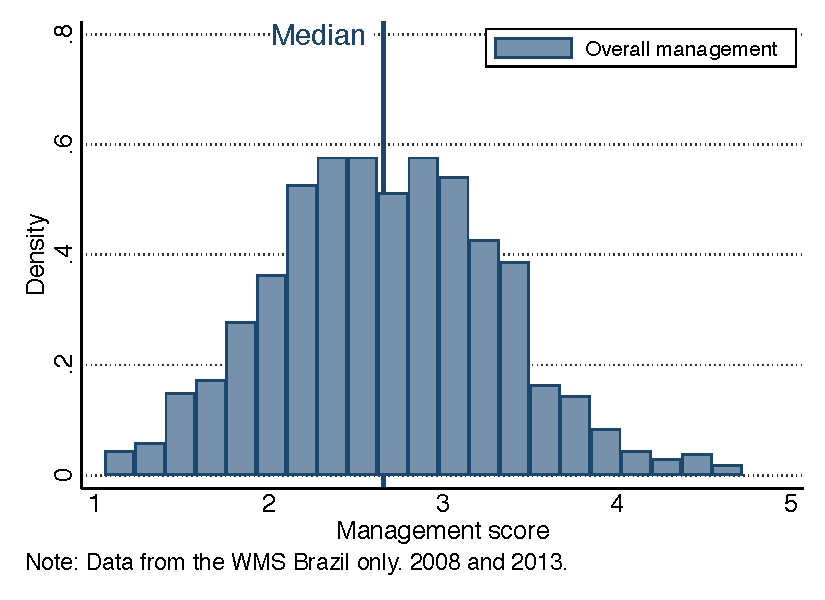
\includegraphics[height=0.75\textheight]{./includes/mgmt_dist1.pdf}    }
\only<2>{        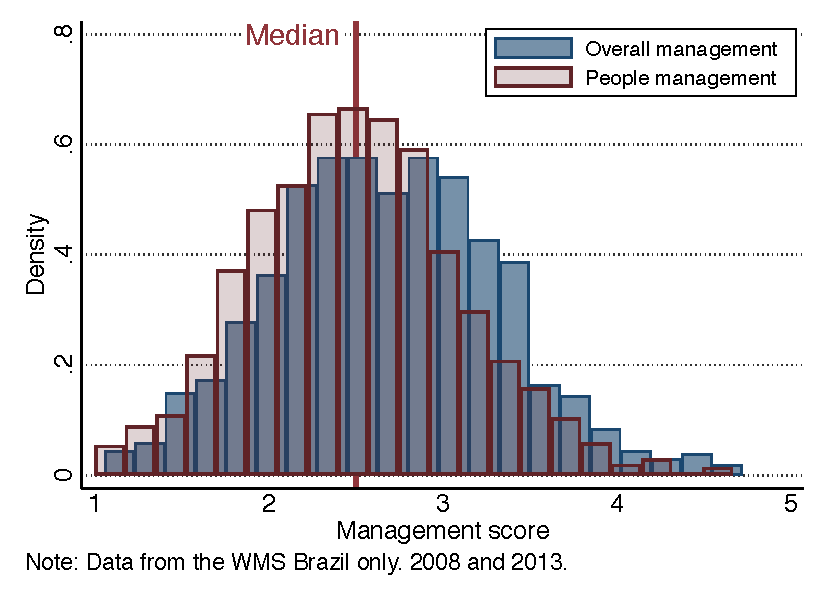
\includegraphics[height=0.75\textheight]{./includes/mgmt_dist2.pdf}    }
\end{frame}
%**********************************************

%**********************************************
\begin{slide}
  \frametitle{A table that is too big}
  \begin{center}
      \scalebox{.45}{
          % !TeX root = ../AER Insights.tex
%tab_prodfcn_2008_old.tex
%Ian M. Schmutte
% 2018-10-29
% Uses results from C:\Users\schmutte\Dropbox\MGMT_source\output\IBGE\tables\ly_collapse.tex

% \begin{table}[h t]
%   \caption{Production Function Estimates: WMS-RAIS-PIA Matched Data} \label{tab:e1_prodfcn}
% \begin{center}
\begin{tabular}{lllll}
    \toprule
                                  & (1)      & (2)       & (3)       & (4)       \\
                                  & ln(sales)& ln(sales)& ln(sales)& ln(sales) \\
    \midrule
z-management                      & 0.088*** & 0.065***  & 0.064***  & 0.059***  \\
                                  & (0.02)   & (0.01)    & (0.01)    & (0.01)    \\
Z-Avg person effect               & 0.076*** &           &           &           \\
                                  & (0.02)   &           &           &           \\
Z-Avg prod worker effect          &          & 0.031**   & 0.028*    & 0.010     \\
                                  &          & (0.02)    & (0.02)    & (0.02)    \\
Z-Avg manager effect              &          & 0.078***  & 0.076***  & 0.053***  \\
                                  &          & (0.02)    & (0.02)    & (0.02)    \\
Share workers with college degree &          &           & 0.05      & 0.05      \\
                                  &          &           & (0.10)    & (0.10)    \\
% Log employees                     & 0.367*** & 0.311***  & 0.311***  & 0.316***  \\
%                                   & (0.04)   & (0.02)    & (0.03)    & (0.02)    \\
% Log capital                       & -0.022** & -0.026**  & -0.026**  & -0.029*** \\
%                                   & (0.01)   & (0.01)    & (0.01)    & (0.01)    \\
% Log materials                     & 0.646*** & 0.701***  & 0.700***  & 0.688***  \\
                                  % & (0.03)   & (0.02)    & (0.02)    & (0.02)    \\
Z-Avg firm effect                 &          &           &           & 0.098***  \\
                                  &          &           &           & (0.02)    \\
Family-owned                      & -0.077** & -0.099*** & -0.098*** & -0.098*** \\
                                  & (0.04)   & (0.03)    & (0.03)    & (0.03)    \\
Founder-owned                     & -0.030   & -0.068*   & -0.068*   & -0.050    \\
                                  & (0.04)   & (0.04)    & (0.04)    & (0.04)    \\
% Industry                          & Yes      & Yes       & Yes       & Yes       \\
\# Observations                   & 773      & 663       & 663       & 663    \\
\# Firms                          & 679      & 594       & 594       & 594    \\
$R^2 $                            & 0.96     & 0.97      & 0.97      & 0.97      \\
\bottomrule
\end{tabular}
% \end{center}

% \end{table}
    
      }
\end{center}
\scalebox{.5}{
\noindent{Controls include: industry, log of capital, raw materials, and the number of employees. 
  }
  }
  You can resize with \texttt{scalebox}
\end{slide}
%**********************************************


%**********************************************
\begin{transitionframe}
  Use this transitionframe environment to set off a new section
\end{transitionframe}
%**********************************************

%**********************************************
\begin{slide}
	\frametitle{Stand-alone figure}
	\begin{center}
		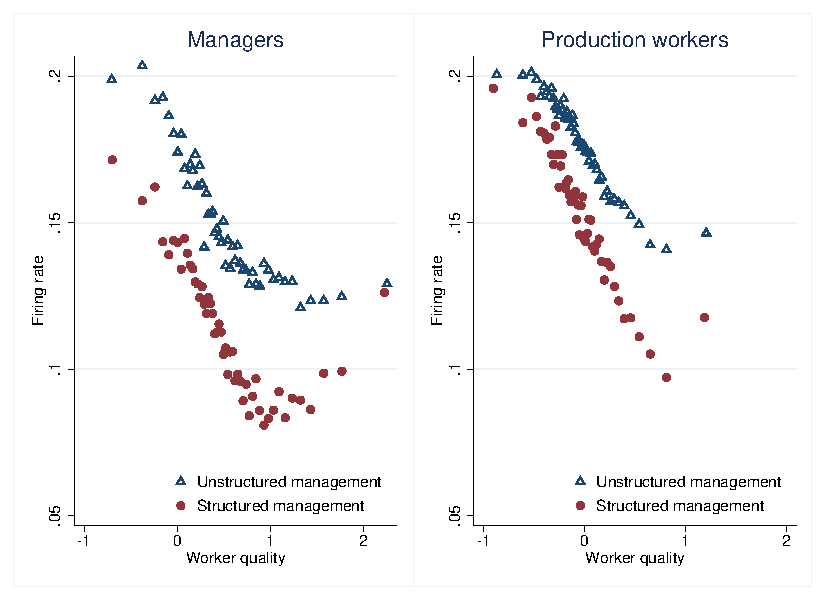
\includegraphics[width = 0.6\textwidth]{./includes/fig_firing_binscatter.pdf}
	\end{center}
\end{slide}
%**********************************************


\begin{slide}
  \bibliographystyle{dcu}
  \bibliography{./references.bib}
\end{slide}

\end{document}

\end{document}










